
我们知道为了有效地使用处理器,必须有足够的代码来并行执行多条指令。没有足够的指令来保持CPU繁忙的主要原因可能是数据依赖,由于输入没有准备好,无法运行指令。通过流水线可以来解决这个问题,但必须事先知道哪些指令将执行。处理这个问题的方法是,根据计算这个条件的历史走向,对是否采用条件分支进行有根据的猜测。猜测越可靠,性能越好。猜测不可靠时,性能会受到严重影响。

所有这些性能问题的根源是条件分支,下一条要执行的指令直到运行时才知道。这个问题的根本解决方案是重写我们的代码,不使用分支,或者更少的分支。这就是\textbf{无分支计算}。

\subsubsubsection{3.8.1\hspace{0.2cm}循环展开}

事实上,这个想法并不新颖。了解了分支影响性能的机制,因此使用循环展开技术来减少分支数量。回到我们最初的代码示例:

\begin{lstlisting}[style=styleCXX]
for (size_t i = 0; i < N; ++i) {
	a1 += p1[i] + p2[i];
}
\end{lstlisting}

虽然循环体是完全流水的,但是这段代码中有一个隐藏的分支:循环检查的结束,这个检查在每个循环迭代中执行一次。若事先知道,迭代次数N是偶数,就不需要在奇数次迭代后执行检查,可以显式地省略这个检查:

\begin{lstlisting}[style=styleCXX]
for (size_t i = 0; i < N; i += 2) {
	a1 += p1[i] + p2[i]
		+ p1[i+1] + p2[i+1];
}
\end{lstlisting}

展开循环,将两个迭代转换为一个更大的迭代。这个例子和其他类似的例子一样,手动展开不太可能提高性能。首先,如果N很大,循环分支的结束部分可以完美地预测出来。其次,编译器可能会将展开作为一种优化,矢量化编译器将使用SSE或AVX指令来实现这个循环。实际上,这里对循环体进行展开的原因是,向量指令一次可以处理多个数组元素,不过这些结论都需要通过基准测试或分析来确认。如果发现手动循环展开对性能没有影响,不要感到惊讶(我们对于分支的理解没有问题),这意味着原始代码已经进行了循环展开,这个优化操作已经由编译器完成了。

\subsubsubsection{3.8.2\hspace{0.2cm}无分支选择}

循环展开是一个非常特殊的优化,编译器会来做这件事。将展开的想法转化为无分支计算是最近的进展,可以带来惊人的性能收益。我们将从一个非常简单的例子开始:

\begin{lstlisting}[style=styleCXX]
unsigned long* p1 = ...; // Data
bool* b1 = ...; // Unpredictable condition
unsigned long a1 = 0, a2 = 0;
for (size_t i = 0; i < N; ++i) {
	if (b1[i]) {
		a1 += p1[i];
	} else {
		a2 += p1[i];
	}
}
\end{lstlisting}

假设条件变量\texttt{b1[i]}不能由处理器预测,这段代码的运行速度比良好的分支预测循环慢几倍。这里可以做得更好,就是可以完全消除这个分支,并通过指向两个目标变量的指针数组,通过索引来进行替换:

\begin{lstlisting}[style=styleCXX]
unsigned long* p1 = ...; // Data
bool* b1 = ...; // Unpredictable condition
unsigned long a1 = 0, a2 = 0;
unsigned long* a[2] = { &a2, &a1 };
for (size_t i = 0; i < N; ++i) {
	a[b1[i]] += p1[i];
}
\end{lstlisting}

转换中,利用了布尔变量只能有两个值(0(\texttt{false})或1(\texttt{true})),将其转换为整数(如果用其他类型代替\texttt{bool},必须确保所有的真值都由1表示,因为任何非零值都认为是真值,但只有1的值在我们的无分支代码中有效)。

这个转换通过对两个内存位置中的一个进行条件访问,替换掉指令中的条件跳转。由于这种条件内存访问可以流水化,无分支的版本具有显著的性能改善:

%\hspace*{\fill} \\ %插入空行
\begin{center}
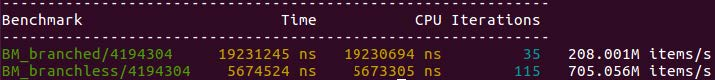
\includegraphics[width=0.9\textwidth]{content/1/chapter3/images/30.jpg}\\
图 3.30
\end{center}

这个例子中,无分支的代码版本要快3.5倍。有些编译器在可能的情况下使用查找数组,而不使用条件分支来实现\texttt{?:}操作符。使用这样的编译器,可以通过如下循环体获得相同性能:

\begin{lstlisting}[style=styleCXX]
for (size_t i = 0; i < N; ++i) {
	(b1[i] ? a1 : a2) += p1[i];
}
\end{lstlisting}

通常,确定这种优化是否有效或效果如何的唯一方法是测试。

前面的例子涵盖了无分支计算的所有基本元素:不是有条件地执行这个或那个代码,而是转换它们,使代码在所有情况下都相同,条件逻辑由索引操作实现。我们将通过更多的例子来强调一些事项和限制。

\subsubsubsection{3.8.3\hspace{0.2cm}无分支的例子}

大多数时候,依赖于条件的代码并不简单。通常,必须根据一些中间值来进行不同的计算:

\begin{lstlisting}[style=styleCXX]
unsigned long *p1 = ..., *p2 = ...; // Data
bool* b1 = ...; // Unpredictable condition
unsigned long a1 = 0, a2 = 0;
for (size_t i = 0; i < N; ++i) {
	if (b1[i]) {
		a1 += p1[i] - p2[i];
	} else {
		a2 += p1[i] * p2[i];
	}
}
\end{lstlisting}

条件影响计算的表达式和结果存储的位置。两个分支唯一的共同之处就是输入,通常情况下,即使是输入也不一定是这样。

为了在没有分支的情况下计算出相同的结果,必须从条件变量索引的内存位置获取正确表达式的结果。因为我们决定不根据条件更改执行的代码,所以两个表达式都将执行。这样,向无分支的转换就很简单了:

\begin{lstlisting}[style=styleCXX]
unsigned long a1 = 0, a2 = 0;
unsigned long* a[2] = { &a2, &a1 };
for (size_t i = 0; i < N; ++i) {
	unsigned long s[2] = { p1[i] * p2[i], p1[i] - p2[i] };
	a[b1[i]] += s[b1[i]];
}
\end{lstlisting}

两个表达式都执行了,结果存储在一个数组中。该数组用于索引计算的目标,即递增的变量。这增加了循环体的计算量,由于是连续的代码,没有了跳转,所以只要CPU有资源做更多的操作,这里的性能就会有提升。基准测试证实了这种无分支转换确实有效:

%\hspace*{\fill} \\ %插入空行
\begin{center}
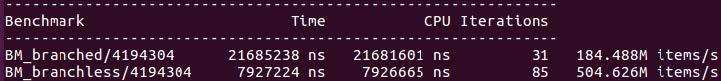
\includegraphics[width=0.9\textwidth]{content/1/chapter3/images/31.jpg}\\
图 3.31
\end{center}

额外计算的数量有限,而且仍然优于条件代码。这里甚至没有一个通用型经验法则可以用来进行猜测(无论如何,都不应该猜测性能)。必须测量这种优化的有效性,它高度依赖于代码和数据。若分支预测器非常有效(可预测的条件,而不是随机条件),那么条件代码将优于无分支的版本:

%\hspace*{\fill} \\ %插入空行
\begin{center}
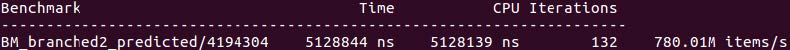
\includegraphics[width=0.9\textwidth]{content/1/chapter3/images/32.jpg}\\
图 3.32
\end{center}

可以从图3.31和图3.32中得到的结论是,流水线刷新(错误预测的分支)的成本有多高,以及CPU在指令级并行性的同时可以做多少计算。无分支计算依赖的是隐藏的和未使用的计算资源,可能还没有耗尽这个资源(在我们的示例中)。我们可以展示代码的无分支转换的另一个版本,不使用数组来选择正确的结果变量,如果不想改变结果,将两者加零:

\begin{lstlisting}[style=styleCXX]
unsigned long a1 = 0, a2 = 0;
for (size_t i = 0; i < N; ++i) {
	unsigned long s1[2] = { 0, p1[i] - p2[i] };
	unsigned long s2[2] = { p1[i] * p2[i], 0 };
	a1 += s1[b1[i]];
	a2 += s2[b1[i]];
}
\end{lstlisting}

现在有两个中间值的数组,而不是目标数组。这个版本会无条件地进行更多的计算,并且具有与之前无分支代码相同的性能:

%\hspace*{\fill} \\ %插入空行
\begin{center}
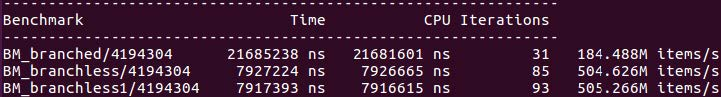
\includegraphics[width=0.9\textwidth]{content/1/chapter3/images/33.jpg}\\
图3.33 - 图3.31的结果,为另一个无分支实现添加了“BM\_branchless1”
\end{center}

理解无分支变换的局限性是很重要的,不要忘乎所以。我们已经看到了一个限制:无分支代码通常要执行更多指令。因此,如果分支预测器工作良好,那么少量的流水刷新可能不足以证明优化的合理性。

无分支转换不能按预期执行的第二个原因与编译器有关:在某些情况下,编译器可以进行等效或更好的优化。例如\textbf{钳位环(clamp loop)}:

\begin{lstlisting}[style=styleCXX]
unsigned char *c = ...; // Random values from 0 to 255
for (size_t i = 0; i < N; ++i) {
	c[i] = (c[i] < 128) ? c[i] : 128;
}
\end{lstlisting}

该循环将\texttt{unsigned char}数组\texttt{c}的值限制为128。初始值是随机的,循环体中的条件在任何程度上都不能预测,可以预期一个非常高的分支错误预测率。另一种无分支的实现使用具有256个元素的\textbf{查找表(LUT)},每个元素对应一个\texttt{unsigned char}值。索引\texttt{i}从0到127的表项\texttt{LUT[i]}包含索引值本身,更高索引值的在\texttt{LUT[i]}中为128:

\begin{lstlisting}[style=styleCXX]
unsigned char *c = ...; // Random values from 0 to 255
unsigned char LUT[256] = { 0, 1, …, 127, 128, 128, … 128 };
for (size_t i = 0; i < N; ++i) {
	c[i] = LUT[c[i]];
}
\end{lstlisting}

大多数现代编译器,这根本不是优化问题:编译器可以更好地处理原始代码,很可能使用SSE或AVX向量指令一次复制和多个钳位字符,从而不需要任何分支。我们对原始代码进行了剖析(而不是假设分支必须错误预测),发现该程序不会受到分支预测的影响。

还有一种情况是,无分支转换可能不成功,即循环体的开销明显高于分支(即使是错误的预测分支)。这种情况值得注意,因为它经常会在循环中使用:

\begin{lstlisting}[style=styleCXX]
unsigned long f1(unsigned long x, unsigned long y);
unsigned long f2(unsigned long x, unsigned long y);
unsigned long *p1 = ..., *p2 = ...; // Data
bool* b1 = ...; // Unpredictable condition
unsigned long a = 0;
for (size_t i = 0; i < N; ++i) {
	if (b1[i]) {
		a += f1(p1[i], p2[i]);
	} else {
		a += f2(p1[i], p2[i]);
	}
}
\end{lstlisting}

根据条件\texttt{b1},我们调用两个函数中的一个,\texttt{f1()}或\texttt{f2()}。如果使用函数指针数组,可以消除\texttt{if-else}语句,可以使代码无分支:

\begin{lstlisting}[style=styleCXX]
decltype(f1)* f[] = { f1, f2 };
for (size_t i = 0; i < N; ++i) {
	a += f[b1[i]](p1[i], p2[i]);
}
\end{lstlisting}

这是值得做的优化吗?通常情况下,并不是。首先,如果可以内联\texttt{f1()}或\texttt{f2()},那么函数指针调用将阻止这种情况。内联通常是一个主要的优化,放弃内联来摆脱分支是不合理的。函数没有内联,函数调用本身就破坏了流水(这是内联是有效的优化的一个原因)。与函数调用的成本相比,即使是一个错误的分支预测通常也没有那么多性能开销。

尽管如此,有时函数查找表也是值得优化的:它从不只提供两个选项,但是如果必须基于一个条件从多个函数中进行选择,那么函数指针表比链式\texttt{if-else}语句更有效。值得注意的是,这个示例与所有现代编译器用于实现虚函数调用的实现非常相似,调用也使用函数指针数组(而不是比较链)。如果需要优化基于运行时条件,调用多个函数中的一个,则应该考虑是否应该使用多态对象进行重新设计。

还应该记住无分支转换对代码可读性的影响:函数指针的查找表不容易读懂,调试起来可能比开关或if-else语句困难得多。由于影响最终结果的因素很多(编译器优化、硬件资源可用性、程序操作数据的属性),任何优化都必须通过基准测试和概要数据文件之类的测量进行验证,并权衡其源码对于开发者的开发时间、可读性和复杂性。






